\chapter{Fundamentals of Classical Information Theory}
\chaptermark{Classical Information Theory}

\par In 1948 Claude E. Shannon published the seminal article “A Mathematical Theory of Communication” exploring the problem of sending information over a communication channel. This was the concrete beginning of classical information theory. This chapter discusses the fundamental ideas of classical information theory. We discuss what information is, how efficiently it can be compressed or sent, and various measures to quantify information.

\par First we need to define exactly what we mean by the term “information”. Usually when people talk about information, they may have different meanings in mind. To some a literary work may have more information than a phone book, to others it may be the other way around. But to devise a formal theory of information we need to have a concrete and quantifiable definition of it.

\section{The Classical Bit}
\par Suppose we are holding an object. Let us ask a question: how much information is contained in this object? To answer the question, we'll have to think about a context in which we need to "transfer" that information to someone else. Let us say we have a friend to whom we need to transfer the complete information of this object. What would that information be? Information in this context will be the size of the set of instructions we need to provide that friend so that he can successfully reconstruct the object.
Suppose the object is an electrical switch and we need to send the information on what state the switch is in. The switch can have one of two possible states: on and off with equal probabilities. The information content we send will be a choice between these two possible alternatives. We call this binary choice a bit - or a binary digit.
\par In general, we can reduce a choice between any number of alternatives to $n$ number of choices between binary alternatives. If we need to make one binary choice between equally probable outcomes then the information content is said to be one bit. If we have to specify between $n$ number of such binary choices then we say the information content is $n$ bits.


\section{Quantifying Classical Information}
The \textit{bit} discussed earlier is a \textit{unit} for information. We now explore the \textit{quantity} - information itself - for which the bit is a unit. To do that we take a look at Shannon's original work on classical information theory.
\par Shannon in his work modeled information as events that happen with certain probabilities. To devise a measure of information he postulated some requirements which any measure of information must fulfill.
\begin{itemize}
\item The amount of information in an event $x$ must depend only upon its probability $p_x$ of happening. In this sense, events that are less likely to happen will carry more information than events that are more likely to happen. We can also say that information is the amount of surprise in an event.
\item Information $I(p)$ is a continuous function of $p$. As we are already familiar, continuity is indeed a desirable quality for physical quantities.
\item $I(p_x,p_y)=I(p_x)+I(p_y)$ which means that information contained in two independent events should be additive.
\end{itemize}
\par Shannon proved that there is indeed a unique measure of information which satisfies these requirements. This measure is unique upto an additive and multiplicative constant. This measure we call the \texttt{Shannon Entropy}.

\subsection{Shannon Entropy}
\par Suppose a message consists of a long string of letters in which each letter $i$ comes from a set of $n$ different letters, each occurring with a probability $p_i$. From requirement 1 it is clear that the information content of the message should depend on $1/p_i$. The less probable the letter, the more surprise you have. To fulfill requirement 3 we choose the function $\log$. Thus the information $I(i)$ in one of the letters $i$ is
\begin{align*}
I(i) = \log\frac{1}{p_i}
\end{align*}
We can see that if we have two events (or two letters), the surprise is additive.
\begin{align*}
I(i,j)= \log(\frac{1}{p_i}\frac{1}{p_j}) = \log\frac{1}{p_i} + \log\frac{1}{p_j}
\end{align*}
The average information contained in a message is the \textbf{Shannon Entropy}.
\begin{align*}
H = \sum_i p_i \log \frac{1}{p_i} = - \sum_i p_i \log p_i
\end{align*}

\subsection{Data Compression}
\par The basic concept of data compression is based on the idea that in any given message there will be redundancy of certain letters or symbols used to encode that message. Such redundancy can always be eliminated by encoding the message more efficiently. In this section we explore the minimum theoretical limit to which we can compress a given message.
\par Suppose we have a long message comprising of a large number $N$ of binary letters. As $N$ gets large enough, $N p_1$ of these letters will be 1's and $N p_0$ letters will be 0's. The number of ways we can arrange these letters is
\begin{align*}
\frac{N!}{(N p_1)!(N p_o)!}
\end{align*}
which are all equally likely to occur.
\par We can label all of them with a binary number. The number of binary digits $I$ we will need to label all these is
\begin{align*}
I = \log_2 (\frac{N!}{(N p_1)!(N p_o)!})
\end{align*}
For a large enough message the original $N$ bits message can be reconstructed with arbitrary precision using just $I$ bits.
Using Stirling's approximation for log of factorials
\begin{align*}
\log(M!) = M \log(M) - M
\end{align*}
We get the relation for information content $I$ of the message
\begin{align*}
I = -N ( p_1 \log p_1 + p_0 \log p_0 )
\end{align*}
which can be generalized to $i$ letters each occurring with probability $p_i$. When we sum them up, we find the familiar expression for Shannon entropy which now also relates to the average information content per symbol.
\begin{align*}
\frac{I}{N} = H\{p_i\} = - \sum_{i=1}^{n} p_i \log p_i
\end{align*}

\section{Capacity of a Noisy Channel}
\par Let's say Alice wants to send Bob a message over a classical information channel. If the channel is noisy then there is a chance that some bits that Alice sends will be flipped and change their original state.

\begin{figure}[h]
  \begin{center}
    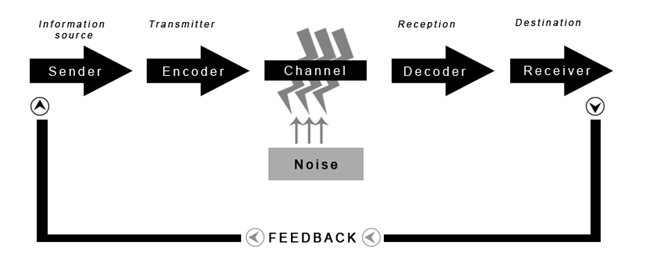
\includegraphics[scale=0.58]{figures/shannon-model-of-communication.png}
    \caption{Shannon's model of communication. A sender encodes some message and transmits it through a channel whereby a receiver receives it and decodes it to access the information that was encoded. Along the channel may exist a source of noise which disrupts the message that was originally sent.}
    \label{fig:}
  \end{center}
\end{figure}

\par We can think of the process like this. What Alice sends is a random variable $X$ and information encoded in that variable. What Bob receives at his end is another random variable $Y$, which depends on both the distribution $X$ and external factors (noise). The information Bob can get out of measuring $Y$ is the mutual information between $X$ and $Y$, $I(X:Y)$. This mutual information is the capacity of that noisy channel. The limit on this capacity is given by Shannon's noisy channel coding theorem.

\subsection{Shannon's Noisy Channel Coding Theorem}
\par If $R$ is the rate of information production and $C$ is the channel capacity, then the information can be transmitted over a noisy channel with arbitrary reliability if
\begin{align*}
R<C=I(X:Y)
\end{align*}
\par If we choose a source that produces information at a greater rate than the channel capacity, then the channel will be unable to handle the information reliably and errors will be inevitable.

